\subsection{Kiến thức về Support Vector Machines (SVM)}
\begin{itemize}
    \item Chọn hàm \textit{Kernel}.
	\item Chọn giá trị điều khiển biến cho dữ liệu huấn luyện C.
	\item Bài toán tối ưu bậc hai để tìm tham số cho vector hỗ trợ.
	\item Xây dựng hàm tách lớp từ các vector hỗ trợ.
\end{itemize}

\subsubsection{Ví dụ minh họa SVM}
\begin{itemize}
    \item Đối với dữ liệu tuyến tính:
    \begin{figure}[H]
        \begin{center}
            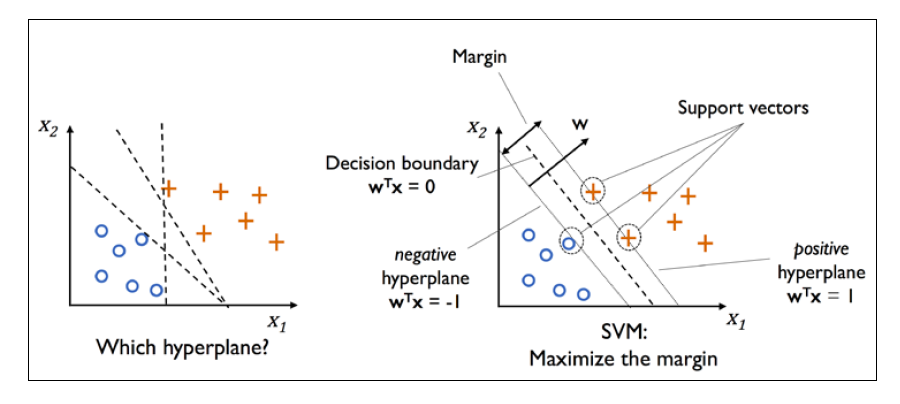
\includegraphics[scale=0.3]{images/theo3/SVM-ex-2}
            \caption{SVM với dữ liệu tuyến tính}
        \end{center}
    \end{figure}

    \item Đối với dữ liệu phi tuyến ta không thể chia trực tiếp bằng các đường thẳng, ta cần phải sử dụng hàm \textit{Kernel} để ánh xạ dữ liệu đó vào không gian nhiều chiều hơn:
    \begin{figure}[H]
        \begin{center}
            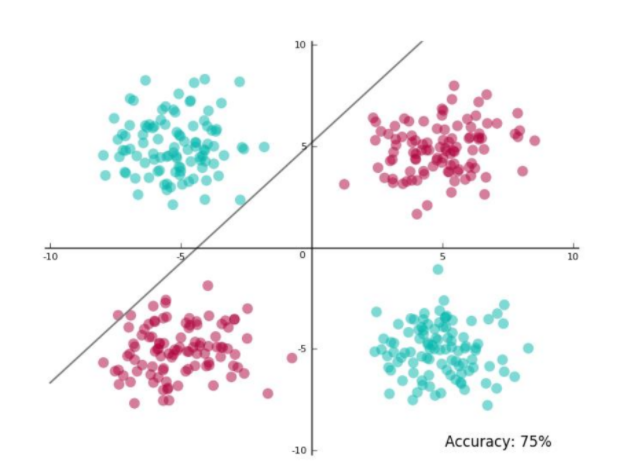
\includegraphics[scale=0.3]{images/theo3/SVM-kernel-1}
            \caption{SVM với dữ liệu phi tuyến}
        \end{center}
    \end{figure}
    \subitem Ta sử dụng hàm \textit{Kernel} để ánh xạ tập dữ liệu 2 chiều trên thành dữ liệu 3 chiều từ đó dễ dàng tìm ra siêu phẳng để phân lớp hơn.
    \begin{figure}[H]
        \begin{center}
            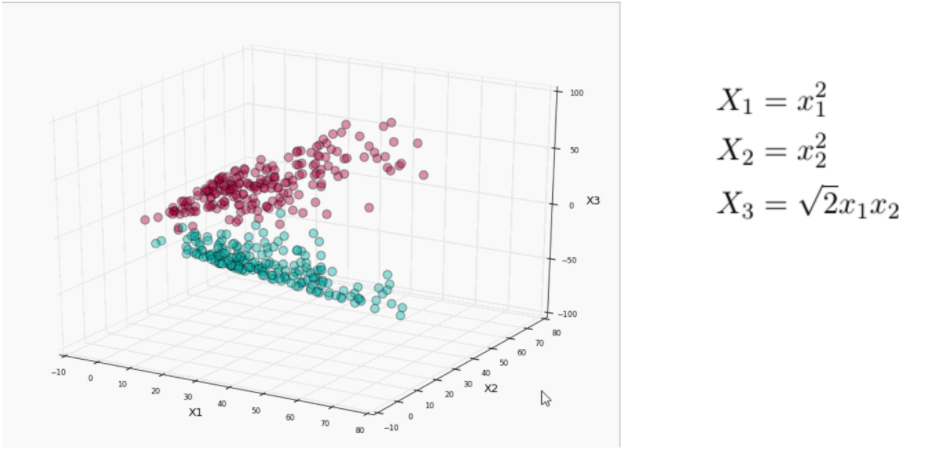
\includegraphics[scale=0.3]{images/theo3/SVM-kernel-2}
            \caption{Tăng chiều dữ liệu bằng các hàm kernel}
        \end{center}
    \end{figure}
\end{itemize}

\subsubsection{Một số hàm kernel thông dụng}
\begin{itemize}
    \item Hàm tuyến tính: $K(x_i, x_j) = x_i^Tx_j$.
    \item Hàm đa thức: $K(x_i, x\_j) = (1 + x_i^Tx_j)^p$
    \item Gaussian: $K(x_i, x_j) = e^{-\frac{\|x_i-x_j\|^2}{2\sigma^2}}$.
    \item Sigmoid: $K(x_i, x_j) = tanh(\beta_0x_i^Tx_j + \beta_1)$
\end{itemize}

\subsubsection{Phân biệt chiến lược one vs all và one vs one}
\begin{itemize}
    \item \textbf{One vs One: }Xây dựng rất nhiều bộ binary classifiers cho từng cặp classes. Bộ thứ nhất phân biệt class 1 và class 2, bộ thứ hai phân biệt class 1 và class 3, … Khi có một dữ liệu mới vào, đưa nó vào toàn bộ các bộ binary classifiers trên. Kết quả cuối cùng có thể được xác định bằng cách xem class nào mà điểm dữ liệu đó được phân vào nhiều nhất (major voting). Như vậy, nếu có C classes thì tổng số binary classifiers phải dùng là n(n – 1)/2. Đây là một con số lớn, cách làm này không lợi về tính toán.
    \item \textbf{One vs All: }Nếu có C classes thì ta sẽ xây dựng C classifiers, mỗi classifier tương ứng với một class. Classifier thứ nhất giúp phân biệt class 1 vs not class 1 , tức xem một điểm có thuộc class 1 hay không, hoặc xác suất để một điểm rơi vào class 1 là bao nhiêu. Tương tự như thế, classifier thứ hai sẽ phân biệt class 2 vs not class 2, … Kết quả cuối cùng có thể được xác định bằng cách xác định class mà một điểm rơi vào với xác suất cao nhất.
\end{itemize}